\chapter{Related Work}

%- Present state of tech (rather state of the art reports)
%    ==> Comparing theory, like the IoT Survey that's a state of the art reports
%    --> Industry is very interested in the IoT/WoT
%    At present Siemens is not so far; Siemens concentrates on B2B solutions
%- How mature is this technology? --> Technology readiness level for WoT, you make the grade use EU Projects for IoT (hint: there are 7)
%- http://iot-epi.eu/
%- What needs to be done still?
%- Haneberg>> Wissenschaftliche Grundlagen erklaeren? zB: RDF, SPARQL, kurz und bundig erklären, use citation numbers, include in References


This chapter will explain some aspects of one of the most important technologies behind the Web of Things, namely the Semantic Web. A cursory description of the Semantic Web will be provided, the reason it was created, and its role in the Web of Things. We will then discuss two main components of the Semantic Web relevant to this work, RDF and SPARQL and how they relate to a major building block in the Web of Things, the Thing Description. An understanding of these technologies will help when we examine the implemented algorithms.

\section{Interoperability}
A key challenge to the WoT is interoperability, sometimes referred to as integration. The term is used to describe the ability for heterogeneous hardware to seamlessly work together in a network. The mission statement of the W3C for the WoT claims, that the WoT is "intended to enable interoperability across IoT Platforms and application domains" by providing the tools to describe, "IoT interfaces". Through such standards, Things could communicate with one another, regardless of their lower-level implementation or their available networking protocols. \cite{Kazuo.2017}

Experts distinguish between two types of interoperability: vertical and horizontal. Vertical interoperability includes interoperability between hierarchies within one domain, whereas horizontal interoperability allows exchange of data between domains. One can imagine vertical interoperability would be the interoperability of Things within a factory, whereas horizontal interoperability is the compatibility between different factories in a supply chain\cite{wang2016implementing}. The goal of the WoT is to provide both types of interoperability and in this work the discovery algorithms are intended to work in a vertical application.

\begin{figure}[th]
\centering
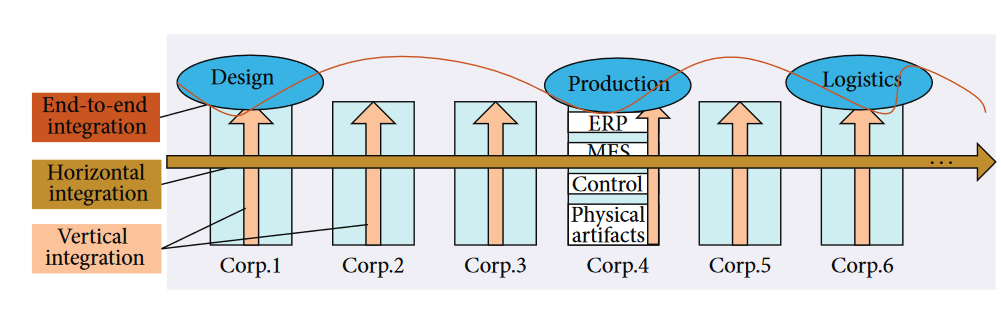
\includegraphics[width=\textwidth]{Figures/integration.png}
\caption{The three types of integration: vertical, horizontal, and end-to-end, as presented in Wang 2016}
\cite{wang2016implementing}
\label{fig:wangIntegration}
\end{figure}

The ultimate goal of the WoT is seamless interoperability in both directions, especially horizontal, e.g. between arbitrarily different domains. By "translating" existing domain standards into machine readable formats instead creating new standards, Things can be connected across and within domains\cite{MichahellesWoS}. Seamless interoperability combined with Industry 4.0 would allow an exhaustive data exchange between all links in a product's supply chain; this is referred to as \textit{end-to-end} interoperability. It would make products and their respective qualities easily reproducible\cite{wang2016implementing}, thus aiding quality control/assurance especially with regards to finding the causes production flaws.

In the example with Tricia and the water reclamation facility, Tricia is charged with designing a system that has vertical interoperability, because she wants to create an integrated smart factory. In an extension of this example, horizontal interoperability would be useful for the integration of the municipal power grid. Let's suppose the reclamation facility has two main power sources aside from the municipal power grid: solar panels and the ability to generate electricity from the decomposing solid waste, raked off before the black water\footnote{waste-water that contains fecal matter.} is processed. It would be useful for the facility to feed power into the gird if there is an abundance of power being generated. Likewise it would help the facility to take advantage of low energy costs, when the municipal grid has a power abundance. As renewable power sources with a stochastic nature, such as wind turbines or solar cells, become more prevalent, this will be more useful, especially since at this scale electricity cannot be effectively stored. Tricia knows this, because she paid attention in her electrical engineering class and is therefore eager to get her plant horizontally integrated.




\section{The Semantic Web}
For the creators of the Web of Things, Dominique D. Guinard and Vlad M. Trifa, it was vital to reuse proven technology to build an architecture for the WoT, rather than develop yet another standard. Guinard and Trifa hoped this would reduce the number of competing standards, thus accelerate the WoT's development. \cite{Guinard.2016}

The cornerstone of the WoT is the Semantic Web. In the way the Web allows users to easily access documents, so should the Semantic Web allow machines to access data. This is the foundation for machine-to-machine (M2M) communication. In May 2001 Tim Berners Lee first openly discussed the Semantic Web in the \textit{Scientific American}. Its purpose was to extend the Web, so that the information found in it can be easily understood by computers for higher level tasks. Lee proposed an extension to the Web, that was decidedly data-centric for machine consumption, to accompany the document-rich Web for humans. At the time he identified three central components to the Semantic Web: XML, RDF, and ontologies. The first two will be discussed below, the last is a way to link two databases that may use different identifiers to connect the same concepts. For example, look at the zip code. Most US citizens will say ZIP code, elsewhere they may prefer postcode or postal code. How machines should understand that these concepts are all the same is tackled by ontologies. \cite{berners2001semantic}

\begin{figure}[th]
\centering
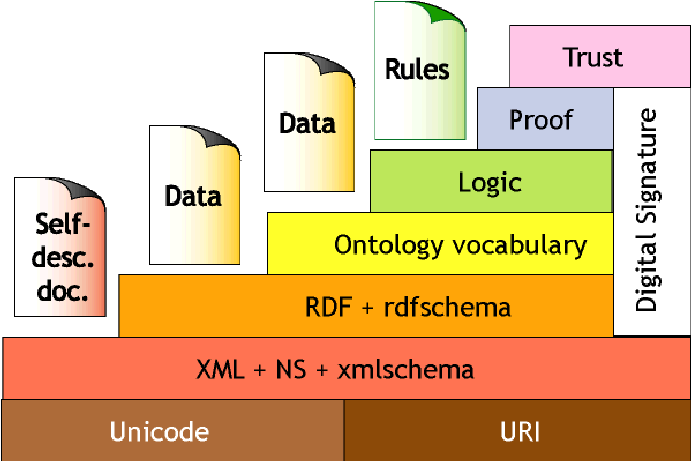
\includegraphics[width=\textwidth]{Figures/SemWebLayer}
\caption{The Semantic Web Layers as Presented by Tim Berners Lee}
\cite{berners2001semantic}
\label{fig:semWebCake}
\end{figure}





Ontologies are a combination of vocabularies and axioms \cite{Cyganiak.2014}. They have vocabularies, taxonomies and inference rules, i.e. a means to define classes and their relationships, and a means to deduce meaning between other ontologies. \cite{berners2001semantic} They can be defined by using the Web Ontology Language (OWL).

The W3C OWL Recommendation defines ontologies as formalized vocabularies with some sort of axiom for describing the nature of relationships. \cite{Synak.2009} \change{this is in the OWL recommendation, not RDF} Ontologies and vocabularies are, to put it curtly, complicated. Semanticists debate their standards and a deep understanding of them surpasses the scope of this work.

In this work the QUDT ontology was used, which describes the relationship between quantities, units, and data types. We only required the vocabularies thereof. The Thing Description is another ontology\cite{Charpenay.2016} this work uses.



%For this work two aspects of the Semantic Web are particularly relevant: RDF for data interchange and SPARQL for querying data.



\section{The Thing Description (TD)}
The Thing Description (TD) is built upon W3C Semantic Web recommendations, specifically the RDF recommendation, which will be discussed in the following section. The success of the WoT depends upon the ability of a Thing to meaningfully expose its capabilities as web resources and interpret the capabilities of other Things\cite{Charpenay.2016}. The TD is currently being drafted and the information is volatile and subject to change, this section refers to the most recently \textit{published} working draft, from April 5, 2018. \change{add this citation, please}


One of these building blocks, the \textit{Thing Description} (TD) standardizes the representation of a Thing's semantic metadata and is analogous the \texttt{index.html} or the landing page of a website. It has not yet been recommended by the W3C, but has only been proposed as a first working draft on September 14, 2017. \cite{Kabisch.2017} \change{add 2018 citation}
Thing Descriptions have been identified as the essential prerequisite for a device to take part in the WoT\cite{Kazuo.2017}. They contain information such as which protocols the Thing supports, which resources and services the Thing has, its geographic location, id, and name. \change{change citation, TD recommendation}


TDs are serialized by default in JSON-LD, a variant of JavaScript Object Notation, and can either be hosted on the Thing itself or elsewhere, when required. Hosting elsewhere is practical when a Thing has limited resources or when legacy devices should be retrofitted to participate in a new WoT system. JSON-LD documents can be serialized in RDF documents due to the mappings between the keywords \texttt{hasThingDescription}, \texttt{hasInteraction}, and \texttt{hasProperty} and \texttt{uris}, \texttt{hrefs}, and \texttt{properties} respectively. The former are contextualized by \url{https://w3c.github.io/wot/w3c-wot-td-context.jsonld}. \change{this can be expanded, love}



Thing Descriptions can be extended by other RDF vocabularies\cite{Kabisch.2017}. In this work the ontology Quantity, Unit, and Data Types (QUDT)\footnote{\url{http://qudt.org/}}, is used to describe the physical units measured by the sensors, like volume and temperature. The ontological model eCl@ssOWL\footnote{\url{http://heppnetz.de/projects/eclassowl/}} was also required. This ontology was generated from industrial standards and characterizes manufactured products. It enables not only the sensors and actuators to be described, but describes the other physical equipment the system entails. Specifically in the FESTO demonstrator this includes the water tanks and pipes.

This work won't go into the details of the used ontologies, because it wasn't especially relevant its contributions and because of the complexity and contreversy surrounding ontologies. Here the reader should just know that there are standard ways to describe resources on the Semantic Web, called ontologies. QUDT is a standard for expressing physical quantities, by standardizing units and ECl@ssOWL allows manufacturers to use\footnote{\uri{www.eclasscontent.com}} standardized metadata for their products.


\change{Add the TD of the LUT400 here, or snippit of it}

Please note, should the principle behind the TD change, this work assumes that a TD is formalized by an RDF graph and is accessed by an interface based off of the W3C SPARQL recommendation, as is currently intended by the TD developers.



\section{The Resource Description Framework (RDF)}
RDF was first recommended by the W3C on February 10, 2004. As the name implies RDF is a framework used to express information about resources. It serves as a data model to facilitate data exchange on the Web. Similarly to Things, resources include documents, various physical objects, people, or even abstract concepts. When information on the Web needs to be processed RDF can be used, since RDF provides a common framework.

RDF provides a way to extend the linking function of the Web by providing the context of a relationship of a link, and not just a connection between its two ends. Therefore, RDF allows developers to make statements about Web resources. The format of which is a triple with the format \texttt{<subject> <predicate> <object>}. Just like a sentence in a natural language, statements express relationships between two entities, namely the \textbf{subject} and the \textbf{object}. The \textbf{predicate} indicates the nature of their relationship. Relationships are directional and told from the perspective of the subject to the object. A simple example is: \texttt{<Jane> <likes> <Richard> .} Recall that the relationship is directional; this means we know Jane likes Richard, but the triple does not imply that Richard likes Jane.

\begin{figure}[th]
\centering
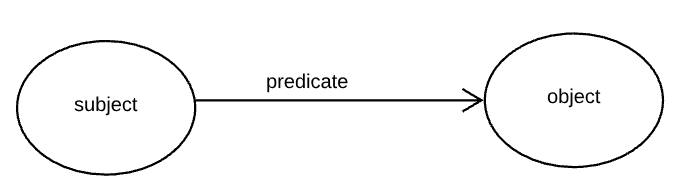
\includegraphics[width=.7\textwidth]{Figures/RDFspo.png}
\caption{RDF data can be represented in graphical form, which is more readable as the data becomes more complex.}
\label{fig:RDFspo}
\end{figure}

Just as sentences can grow in complexity, so can RDF data. It is therefore useful to have different representations of RDF data. Triples, as they appear above can be represented in a graph, which is possibly the simplest mental model. In this model subjects and objects are represented as nodes and the predicates are directed arcs. This is clearly demonstrated in Figure \ref{fig:RDFspo}. A more complicated example of triples is found in Figures \ref{fig:lut400_n-triples} and \ref{fig:rdflut400}, which show the same semantic data from the SITRANS LUT400. They contain elements, that will shortly be explained, but both express exactly the same semantic data for the water level sensor used in the FESTO water management unit. Semantically, there is absolutely no difference between the two, yet the graph is much more readable.


\begin{figure}[ht!]
	\centering
    \fontfamily{pcr}\selectfont
    \begin{tabular}{ l l l }
    <urn:tank1> & <rdf:type> & <ec:C\_AH632010-gen>. \\
    <urn:tank1> & <ex:embeds> & \_:b1. \\
    \_:b1 & <rdf:type> & <ec:C\_AG59007-gen>. \\
    \_:b1 & <wot:hasProperty> & \_:b2. \\
	\_:b2 & <qudt:unit> & <unit:CubicMeter>. \\
	\_:b2 & <qudt:hasQuanityKind> & <quantity:Volume>. \\
	\_:b2 & <wot:hastInteraction> & <coap://192.168.2.61:5683/levelvalue>. \\
	\_:b2 & <rdf:type> & <qudt:Quantity>.
    \end{tabular}

  \caption{Triples from the SITRANS LUT400 water level sensor, which was used in the FESTO Unit.}
  \label{fig:lut400_n-triples}
\end{figure}

So it's clear how RDF data is connected, but not yet clear what the components of an RDF triple are. So what are subjects, objects, and predicates? How can we use them? A resource can be mentioned both as a subject and an object in numerous triples, though not reflexively, e.g. \texttt{<Donald Trump> <loves> <Donald Trump> .} is not allowed.  Subjects, predicates, and objects can be IRIs (Internationalized Resource Identifiers), whereas subjects and objects may be \textit{blank} nodes (more about those in \ref{sec:blanknodes}). Objects may additionally be \textit{literals}, which are used for static values entailing strings, numbers, or dates. Blank nodes, IRIs, and literals are so-called RDF terms. \cite{Cyganiak.2014}

RDF terms are unique and are not equivalent to each other. For example, the IRI \url{www.zombo.com} is not equivalent to the string literal value of \url{www.zombo.com}, and neither are equivalent to the blank node identifier \url{www.zombo.com} \cite{Cyganiak.2014}.  This is important to note when creating semantic data for a Thing, but in this work semantic data was provided, so it will not be explained in further detail.  \change{this sounds like a cop-out}

An example of a literal can be seen in an extension the LUT400 semantic data as seen in Figure \ref{fig:rdflut400}. In the lower right corner there is the resource \texttt{unit:CubicMeter} from the QUDT ontology, on QUDT page for this resource there is the option to add the abbreviation m\textasciicircum3, which is a \texttt{xsd:string}\footnote{\url{http://www.qudt.org/qudt/owl/1.0.0/unit/Instances.html\#CubicMeter}} and therefore a literal. It would be extended by added an arc with the value \texttt{qudt:abbreviation} and would have the aforementioned literal value.

Ontologies are very similar to RDF, which also describes the relationship between objects, in fact each ontology can be described by an RDF graph. The main difference between the two being: RDF describes the relationship between individual objects and ontologies the nature of relationships between \textit{classes} of objects. \cite{Synak.2009}

\change{Explain the graph}

\begin{figure}[th]
\centering
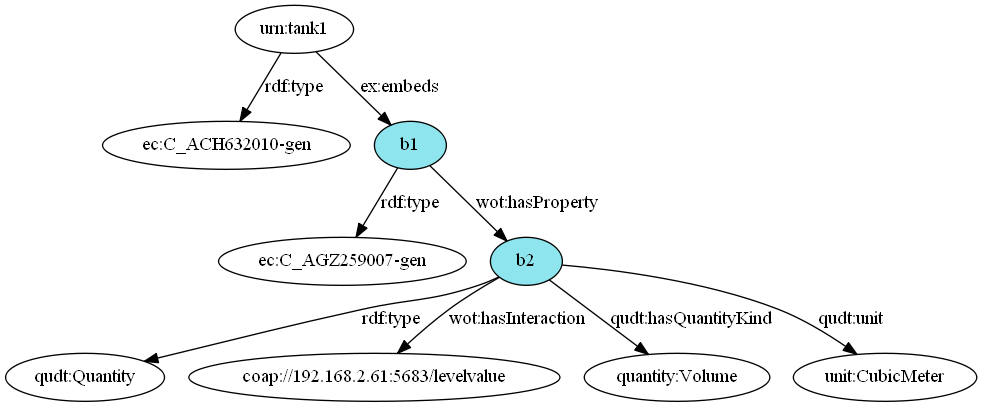
\includegraphics[width=\textwidth]{Figures/lut400}
\caption[The RDF Graph for the LUT400]{RDF Graph of the SITRANS LUT400.}
\label{fig:rdflut400}
\end{figure}


\change{How much information is enough, can additional resources go here?}
\change{Add W3C citation}

\subsection{Blank Nodes}
\label{sec:blanknodes}
Sometimes a node contains neither a resource nor a literal, such nodes are referred to \textit{blank} nodes, sometimes \textit{bnodes}. To see an example of blank nodes, please see Figure \ref{fig:rdflut400}, notice that the blank nodes, in blue, organize the properties of the LUT400 water level sensor and make the RDF graph more readable. Blank nodes can represent complex attributes of other objects\cite{chen2012blank}. E.g. a blank node may be used to organize attributes of an address, which has a postal code, a street name, a city, state/province, a house number, etc. As a part of the RDF standard they represent a core component of the Semantic Web. A 2011 survey found that a majority of the semantic data on the Web contained blank node structures, a minority thereof were complex structures, which are costly to manipulate. \cite{Mallea.2011}

Alarmingly, blank nodes have not been handled consistently by the Semantic Web developers communities; there is a discrepancy between the standard and the implementation. Various serializations of RDF represent blank nodes in unique ways, which makes this problematic for their respective parsers. SPARQL, the query language for RDF regards blank nodes as query variables, which is helpful for the discovery algorithm, since it means that the semantic does not change.

\change{define unlean and connected graphs before this}
\change{blank nodes + OWL = yucky, because when a node has 2 properties, like graphs may be considered unlean in one ontology}
Blank nodes can be problematic: graphs that contain blank nodes and entail joined ontologies may appear unlean, even when it contains no blank nodes. \cite{Hogan.2014} The framework used in this work, Apache Jena, provides methods to compare RDF-graph equivalency. The basis of our this work, requires that graphs do not come from mixed ontologies, because the building of leaned, connected graphs is the foundation of the discovery algorithms. This will be clarified in the next section, where the discovery algorithms are discussed.


\section{RDF Serializations}
RDF describes a graph and as such the representation in computer memory may vary.\cite{Cyganiak.2014} There are many serializations of RDF, but the most common are N-Triples, RDF/XML, and Turtle.


\subsection{N-Triples}
N-Triples is one of the simplest plain-text encodings of an RDF graph. It was originally meant for creating quick RDF test cases, but is now commonly used as an exchange format for RDF data.

N-Triples have a simple subject-predicate-object syntax. RDF IRIs are written in angle brackets and separated by a space, the end of each triple is denoted by a period. Assuming there are no blank nodes in the triple, it would look like this: \texttt{<subject> <predicated> <object> .} Literals are noted by the delimiter \texttt{"} on either side of the literal.

Triples are separated by a new line, which is optional at the end of a document. Comments may be added at the end of each line by using a pound sign (\texttt{\#}). \cite{.02.10.2017c} Looking at N-Triples, it's quite clear why it has become so popular; it has a flat learning curve and it is very quick to generate sample data for testing with.

Figure \ref{fig:lut400_n-triples} shows the LUT400's semantic data written in N-triple format.

\subsection{RDF/XML}

RDF/XML is the format most often associated with RDF, in fact the two are often, incorrectly used interchangeably\cite{Hogan.2014}. The W3C first recommended the serialization in 2004 and then revised their recommendation in 2014\cite{RDFXML.02.10.2017}.

The RDF/XML recommendation defines an XML syntax for RDF graphs to be encoded. Triples can be written a number of ways\cite{RDFXML.02.10.2017}, but basically it works as bellow. Listing \ref{lis:xmlspo} shows the simple s,p,o-triple from figure \ref{fig:RDFspo} in two different RDF/XML notations. The second of which, resemles the format for the LUT400 XML data used in the FESTO unit.

\begin{lstlisting}[language=XML, caption={A trivial RDF triple in RDF/XML}, label={lis:xmlspo}]
<rdf:Description rdf:about="subject">
    <examplenamespace:predicate>
        <rdf:Description rdf:about="object/>
    </examplenamespace:predicate>
</rdf:Description>

<rdf:Description rdf:about="subject">
    <expredicatenamespace:predicate rdf:about="object" />
</rdf:Description>
\end{lstlisting}
\vspace{1cm}

RDF/XML uses Qualified Names (QNames) as its namespace in order to represent IRIs. \change{maybe explain QNames a little more in the RDF section, since this is in common with all serializations}

Compare figures \ref{fig:rdflut400} and \ref{fig:rdfxml}. The first line is like any other XML document, the second is unique to RDF/XML. The graph serialization is typically contained within the \texttt{<rdf:RDF>} and \texttt{</rdf:RDF>} tags. Within the first XML element the namespaces are defined. This works just the same as XML and ensures that there are no naming conflicts. In figure \ref{fig:rdfxml} there are four declared namespaces, which have the prefixes \texttt{demo, qudt, rdf, wot} the first two are needed specifically in the FESTO case. The next element in this figure follows the schema above for the triples and corresponds to \texttt{b1} in figure \ref{fig:rdflut400}. There are two arcs coming out of \texttt{b1}, one goes to \texttt{b2} and is labeled with the predicate names \texttt{wot:hasProperty} and the second points to a web resource with the predicate \textt{rdf:type}. Note that the style of the triple is slightly different in figure \ref{fig:rdfxml} as it is in listing \ref{lis:xmlspo}, this is the same as it would be in normal XML.      \cite{RDFXML.02.10.2017}




\begin{figure}[th]
	\centering
	\resizebox{\textwidth}{!}{\lstinputlisting[language=XML]{Code/lut400.xml}}
    \caption{The LUT400's semantic data represented in RDF/XML format.}
    \label{fig:rdfxml}
\end{figure}



Not all RDF graphs can be serialized using the RDF/XML standard, specially those that use the \textt{rdf:HTML} datatype, those that use reserved names as properties, or those that use property names, which cannot be transformed into XML namespace qualified names, e.g. because they contain characters that are not qualified for QName namespaces \cite{RDFXML.02.10.2017}. RDF/XML documents can be validated using a tool\footnote{https://www.w3.org/RDF/Validator/} provided by the W3C.


\subsection{EXI}
XML is a costly representation of RDF data and embedded devices often do not have the resources to store and process XML. As a result Semantic Web/Linked Data technologies have failed to gain wide-spread traction. To confront this problem researchers at the Siemens Corporate Technology created a solution based off the W3C EXI format. \cite{Kabisch.2015}

The Efficient XML Interchange (EXI) format was formally recommended by the W3C in 2014, and helps to accelerate the exchange of XML data. EXI puts the responsibility of parsing on the server, to which parsing events are sent. It was intended to stream XML data in a without losing any information, unlike RDSZ (The RDF Differential Stream Compressor based on Zlib), with which the RDF structure is lost. This is especially useful when used together with microcontrollers \cite{Kabisch.2015} and when combined with the The Constrained Application Protocol (CoAP) \cite{castellani2011web}.

As defined in the W3C EXI recommendation, an \textit{EXI stream} "is an EXI header followed by an \textit{EXI body}", which "carries the content of the document, while the EXI header communicates the options used for encoding the EXI body" and is therefore necessary to decode the body. The EXI body is composed of so-called EXI events, which encode XML elements. Below is a list of the EXI events with their descriptions. \cite{.02.10.2017b}


\begin{itemize}

\item \textbf{SD}: Starts the EXI stream with a \textbf{S}tart \textbf{D}ocument event.
\item \textbf{NS}: Sets the \textbf{n}ame\textbf{s}pace of the document.
\item \textbf{SE}: A \textbf{s}tart \textbf{e}lement event, which is used to start the element of an XML document.
\item \textbf{AT}: The \textbf{at}tribute event denotes an attribute in XML.
\item \textbf{CH}: The \textbf{ch}aracter event denotes a literal.
\item \textbf{EE}: An \textbf{e}nd \textbf{e}lement event, which follows an SE event. This ends the processing of the current element. This event does not refer to the element, like in XML.
\item \textbf{ED}: Ends the document stream with a \textbf{E}nd \textbf{D}ocument event.
\end{itemize}

XML documents can be described using these events. We can again examine this in the semantic data from the LUT400 water level sensor. Looking at listing \ref{lstEXI}, it is easy to see, how the EXI events correspond to the XML data in figure \ref{fig:rdfxml}. These events appear uncompressed, in reality they would be byte compressed in a way similar to Huffman encoding and the namespaces work the same way the QNames work in XML\cite{.02.10.2017b}.



\begin{lstlisting}[caption={The LUT400's XML data as serialized in EXI events.},captionpos=b, label={lstEXI}]
SD
SE	rdf:RDF
NS	xmlns:demo="http://siemens.com/urdf/ns#"
NS	xmlns:qudt="http://qudt.org/schema/qudt#"
NS	xmlns:rdf="http://www.w3.org/1999/02/22-rdf-syntax-ns#"
NS	xmlns:wot="http://w3c.github.io/wot/wot.owl#"
SE	rdf:Description
AT	rdf:nodeID="f8a04ac1a47924de7ad18c3b413895565b1"
SE	wot:hasProperty
AT	rdf:nodeID="f8a04ac1a47924de7ad18c3b413895565b2"
EE
SE	rdf:type
AT	rdf:resource="http://www.eclass.eu/#C_AGZ259007-gen"
EE
EE
SE	rdf:Description
AT	rdf:nodeID="f8a04ac1a47924de7ad18c3b413895565b2"
SE	wot:hasInteraction
AT	rdf:resource="coap://192.168.2.61:5683/levelvalue"
EE
SE	qudt:unit
AT	rdf:resource="http://qudt.org/vocab/unit#CubicMeter"
EE
SE	qudt:hasQuantityKind
AT	rdf:resource="http://qudt.org/vocab/quantity#Volume"
EE
EE
SE	rdf:Description
AT	rdf:about="http://tank1
SE	rdf:type
AT	rdf:resource="http://www.eclass.eu/#C_ACH632010-gen"
EE
SE	demo:embeds
AT	rdf:nodeID="f8a04ac1a47924de7ad18c3b413895565b1"
EE
EE
EE
ED
\end{lstlisting}



In this work EXI was used to encode semantic data in the XML format. For example, the LUT400's semantic data is 1,098 Bytes in XML vs only XXXXXX in EXI.\change{Size of LUT 400 in EXI}


\subsection{Turtle}
Another syntax for RDF is Turtle: the Terse RDF Triple Language. It is a compact way of expressing RDF and written in an intuitive way. Turtle is compatible with the N-Triples format and the triple pattern specified by the W3C SPARQL recommendation.
\change{are each really written in brackets?}
Like N-Triples, simple triples have the same format: subjects, predicates, and objects are written in that order, each within angled brackets, if they are IRIs. Line comments are also denoted by a \texttt{\#}. Just like in N-Triples, literals are written in quotation marks.

Where Turtle diverges from N-Triples, is in its predicate and object lists. Often the same subjects are referenced in a number of triples. Predicate lists are separated by a semicolon \texttt{;}, whereas object lists are separated by a comma.

\begin{figure}[th]
	\centering
	\begin{lstlisting}[
    basicstyle=\small
]
@prefix rdf:       <http://www.w3.org/1999/02/22-rdf-syntax-ns#> .
@prefix qudt:      <http://qudt.org/schema/qudt#> .
@prefix quantity:  <http://qudt.org/vocab/quantity#> .
@prefix unit:      <http://qudt.org/vocab/unit#> .
@prefix eco:       <http://www.eclass.eu/#> .
@prefix gr:        <http://purl.org/goodrelations/v1#>.
@prefix wot:       <http://w3c.github.io/wot/wot.owl#> .
@prefix demo:      <http://siemens.com/urdf/ns#> .

<http://tank1> a eco:C_ACH632010-gen ; # This is a predicate list
            demo:embeds _:levelsensor .

_:levelsensor a eco:C_AGZ259007-gen ;
              wot:hasProperty _:level .

_:level a qudt:Quantity ;
        wot:hasInteraction <coap://192.168.2.61:5683/levelvalue> ;
        qudt:hasQuantityKind quantity:Volume ;
        qudt:unit unit:CubicMeter .
	\end{lstlisting}
    \caption{The LUT400's semantic data represented in Turtle format}
\end{figure}

Blank nodes in Turtle are denoted by \texttt{\_:} followed by its blank node label.

\cite{Beckett.23.01.2018}

\section{SPARQL}
With RDF semantic data can be represented, but that is nearly useless unless one has a way to query this data.  For example retrieving \url{http://www.munich.de/parking#} could provide data on parking spaces in Munich, which in turn can be identified by their International Resource Identifier (IRI). \cite{Cyganiak.2014} But what really interests someone looking for a parking space is its high-level state: is it free? Does that space include a charging station?


The SPARQL  Protocol and RDF Query Language (SPARQL), pronounced "sparkle", is for querying semantic databases and manipulating RDF data. It was formally recommended by the W3C in 2008  \cite{Herman.2008} and has since been an integral part of the Semantic Web. Tim Berners Lee, the director of the W3C and founder of the Web once said, "Trying to use the Semantic Web without SPARQL is like trying to use a relational database without SQL." \cite{Herman.2008} SPARQL offers tools for querying and analyzing triple patterns and has a similar syntax to SQL. The result of a SPARQL query may be an RDF graph or a result set.

Again, consider the LUT400. Below is a sample query on the LUT400's data, which selects all triples with the predicate \texttt{wot:hasProperty}.

\begin{lstlisting}[
    basicstyle=\small, caption={A sample SPARQL query on the LUT400's data.}, label={lst:QueryLUT400}]
PREFIX wot: <http://w3c.github.io/wot/wot.owl#>
SELECT *
WHERE {
    ?subject wot:hasProperty ?object .
}
\end{lstlisting}

SPARQL Queries can also be used to compare quantities. Suppose there were two LUT400s built into the FESTO unit, labeled by the simple IDs \texttt{1} and \texttt{2}. The \textt{ASK} command returns either \texttt{TRUE} or \texttt{FALSE} if the query has any matching patterns. The query is formed by asking the web resource of the tank about the property of the water level, and these two results from each web resource is compared. \cite{.02Oct17}

\begin{lstlisting}[
    basicstyle=\small, caption={Comparing Volume using a SPARQL query}, label={lst:ASKQueryLUT400}]
PREFIX wot: <http://w3c.github.io/wot/wot.owl#>
ASK {
    <http://example.com/waterlevelsensorID/1> ?wot:hasInteraction ?levelValue1
    <http://example.com/waterlevelsensorID/2> ?wot:hasInteraction ?levelValue2
    FILTER (?levelValue1 > ?levelValue2) .
}

\end{lstlisting}
